\section{Related Work}

In this section, we describe the current approaches for indexing RDF data,
before reviewing the existing search models for (semi) structured data.

\subsection{Retrieval of RDF Data}

The growth of RDF data incurs the need of efficient and scalable data
management systems. Several systems have been proposed based on Relational
DataBases Management Systems (RDBMS)~\cite{beckett:2003:swss-rdbms}. RDF data
management systems are able to store a large amount of data and use SPARQL as a
query language which allows to perform complex searches over the collection. A
user is able to perform complex request when the database schema is known.
However given the heterogeneous data collection on the web, the added value of
SPARQL is limited. Indeed it is difficult to write precise queries since the
data structure and the ontology may vary from one dataset to an other.

Other
approaches~\cite{guha:2003:tap,ding:2005:swoogle,harth:2008:swse,cheng:2008:falcons}
carried over keyword-based search to Semantic Web and RDF data in order to
provide ranked retrieval using content-based relevance estimation. In
addition, such systems are easier to scale due to the simplicity of their
indexing scheme. However, such systems are restricted to keyword search and do
not support structural constraints. These systems do not consider the rich
structure provided by RDF data.

A first step towards a more powerful search
interface combining imprecise keyword search with precise structural
constraints has been investigated by Semplore~\cite{wang:2009:semplore}.
Semplore has extended inverted index to encode RDF
graph approximations and to support keyword-based tree-shaped queries over RDF
graphs. However the increase of query capabilities comes at a cost, and the
scalability of the system becomes limited.

\subsection{Search Models for (semi) Structured Data}

In addition to standardised query languages such as SPARQL, a
large number of search models for semi-structured data have been developed. Some
of them focus on searching structured
databases~\cite{agrawal:2002:dbxplorer,bhalotia:2002:banks,hristidis:2002:discover,liu:2006:sigmod},
XML documents~\cite{cohen:2003:xsearch,guo:2003:xrank,liu:2007:xseek} or
graph-based data~\cite{abiteboul:1996:lorel,kachiola:2005:vldb,li:2008:ease}
using simple keyword search. Simple keyword-based search has the advantages of
\begin{inparaenum}[(1)]
\item being easy to use by users since it hides from the user any structural
information of the underlying data collection, and
\item of being applicable on any scenarios. 
\end{inparaenum}
On the other hand, the keyword-based approach suffers from limited capability
of expressing various degrees of structure when users have a partial knowledge
about the data structure.

Other
works~\cite{kasneci:2008:naga,mandreoli:2009:edbt,wang:2009:semplore,dong:2007:sigmod,fletcher:2009:theory-search}
have extended simple keyword-based search with structured queries
capabilities. \cite{dong:2007:sigmod,fletcher:2009:theory-search} propose a
partial solution to the lack of expressiveness of the keyword-based approach
by allowing search using conditions on attributes and values.
\cite{kasneci:2008:naga,mandreoli:2009:edbt,wang:2009:semplore} present more
powerful query language by adopting a graph-based model. However, the increase
of query expressiveness is tied with the processing complexity, and the
graph-based models
\cite{kasneci:2008:naga,mandreoli:2009:edbt,wang:2009:semplore} are not
applicable on a very large scale.

The search model introduced in Section~\ref{sec:siren-model} is similar to
\cite{dong:2007:sigmod,fletcher:2009:theory-search}, i.e., it is defined
around the concept of attribute-value pairs. However, our model is more
expressive since it differentiates between single and multi-valued attributes
and it considers the provenance of the information.

\section{Formal Model}
\label{sec:siren-model}

The expansion of Semantic Web applications has increased considerably and it
will continue on this progression. A wide range of different technologies has
been developed to represent and use semantic data. For the purpose of covering
a majority of data sources when searching for entities, a formal model has been
introduced. In this section, I give a summary of a labeled directed graph
model, before describing its query model.

\subsection{Entity Attribute-Value Model}

Semantic data can be used to describe any kind of data, from a physical person
to an abstract notion. These \emph{entities} are at the core of any data and
are the unit that is to be searched for with SIREn. This section presents
fundamentals about the Entity Attribute-Value model, a generic model which goal
is to support scenarios involving entities.

A Semantic graph (e.g. a RDF graph) is a graph that gives information about
several entities somehow related to each other. This graph can then be split
into sub-graphs, each one describing a particular entity. A \emph{star graph},
i.e., an entity at the center with associated incoming and outgoing relations.
For instance, the RDF graph in Figure~\ref{fig:rdf-graph} can be split into
three entities, as depicted in the Figure~\ref{fig:entities}. The graph
describing ``The Lord of the Rings'' work is divided into the
\emph{\url{http://dbpedia.org/page/The_Lord_of_the_Rings}}, \emph{\_:bnode1}
and \emph{dbpedia:J.\_R.\_R.\_Tolkien} entities.
% Also, the FOAF file from the
% Listing~\ref{lst:foaf} can be splitted into three entities: \emph{Giovanni
% Tummarello}, \emph{Renaud Delbru} and \emph{Stephane Campinas}.
The star graph gives information about the entity and is then generically
called an \emph{entity description}.

A \emph{dataset} is a source of semantic data, such as a domain or a site web
and it gives the \emph{context} of the data it contains. An \emph{attribute}
refers to the relation between an entity and an object, e.g. the predicate in
a RDF triple. For example ``dbpedia-owl:author'', ``dbpedia-owl:abstract'' and
``dbpprop:precededBy'' are the attributes associated with the \_:bnode1
entity. An attribute can also be \emph{multi-valued} as a book can have
multiple authors for instance. A \emph{value} refers to the node related to an
entity.

\begin{figure}
\centering
\resizebox{\linewidth}{!}{%
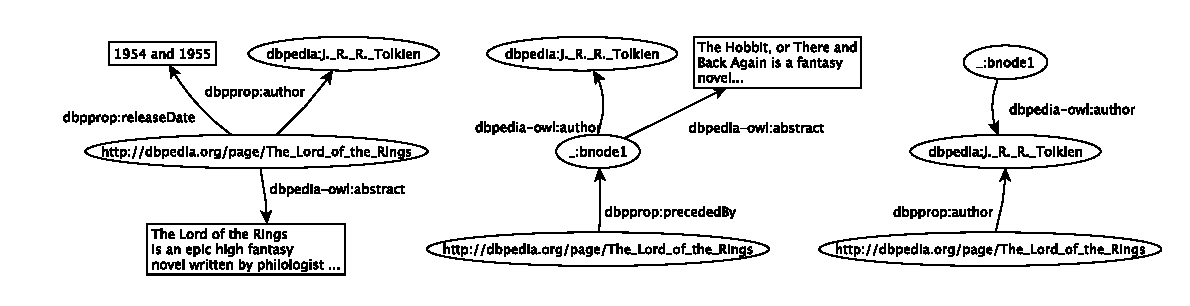
\includegraphics[scale=1]{pics/entities}
}%
\caption{A representation of the RDF graph in Figure~\ref{fig:rdf-graph}
divided into three entities: \emph{The Lord of the Rings}, \emph{\_:bnode1}
and \emph{Tolkien}.}
\label{fig:entities}
\end{figure}

\subsubsection{Node-Labelled Tree Model for RDF}

SIREn uses a node-labelled tree structure to capture the relationship between
values, attributes, entities and datasets. Taking the RDF data model (the
triple) as a support, the tree represent four kinds of nodes as depicted in the
Figure~\ref{fig:tree-model}:
\begin{itemize}
  \item the \emph{dataset} that indicates the context of the data.
  \item the \emph{entity} (the subject).
  \item the \emph{attribute} (the predicate).
  \item the \emph{value} (the object).
\end{itemize}
Each node can refer to one or more terms. In the case of RDF, a term is not
necessarily a word from a literal, but can be an URI or a local blank node
identifier.

A node-labelled tree model enables to encode and efficiently establish
relationships between the nodes of a tree. The two main types of relations are
Parent-Child and Ancestor-Descendant. To support these relations, the
requirement is to assign \emph{unique identifiers}, called node labels, that
encode the relationships between the nodes. The Dewey
encoding~\cite{beyer:2002:ordered-xml} is a simple node labelling scheme. In
Dewey Order encoding, each node is assigned a vector that represents the path
from the tree’s root to the node and each component of the path represents the
local order of an ancestor node. Using this labelling scheme, structural
relationships between elements can be determined efficiently. An element u is
an ancestor of an element v if label(u) is a prefix of label(v). The
Figure~\ref{fig:dewey-encoding} depicts the tree representation of the RDF
graph in Figure~\ref{fig:rdf-graph} using the Dewey encoding. The dataset is
the domain of the URI the graph is hosted at. In that representation, the
qualified names (i.e., QNames) have been removed in order to keep only the
property name, for clarity purpose since the property has the same semantic
even if the QNames are different (e.g., dbpprop:author and dbpedia-owl:author).
For example the entity ``The\_Lord\_of\_the\_Rings'' with vector [1.1], we can
find that it is a parent of the value node ``J.R.R.\_Tolkien'' with vector is
[1.1.2.1].

\begin{figure}
\centering
\subfloat[Conceptual representation of the node-labelled tree model.]{
\resizebox{0.34\linewidth}{!}{%
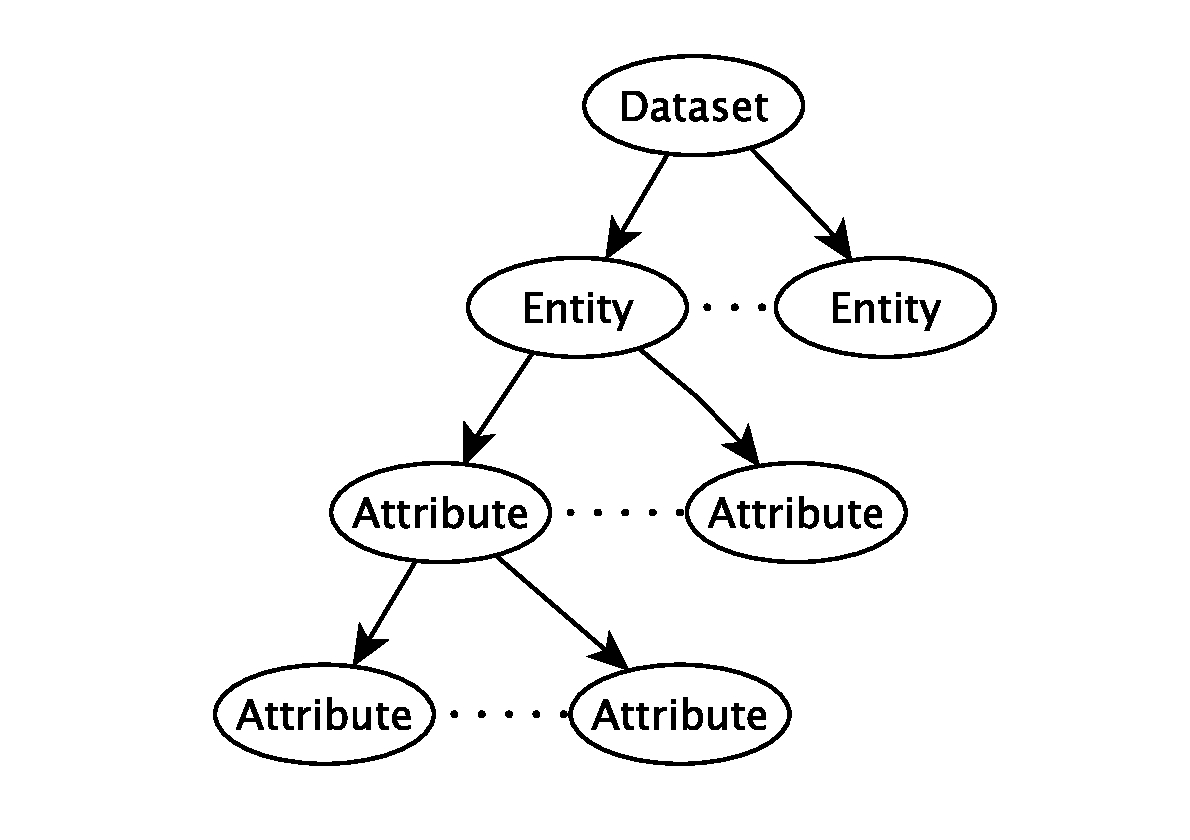
\includegraphics[scale=1]{pics/tree-model}
\label{fig:tree-model}
}}\quad
\subfloat[Node-labelled tree model with Dewey encoding of the dataset in
Figure~\ref{fig:rdf-graph}.]{
\resizebox{0.6\linewidth}{!}{%
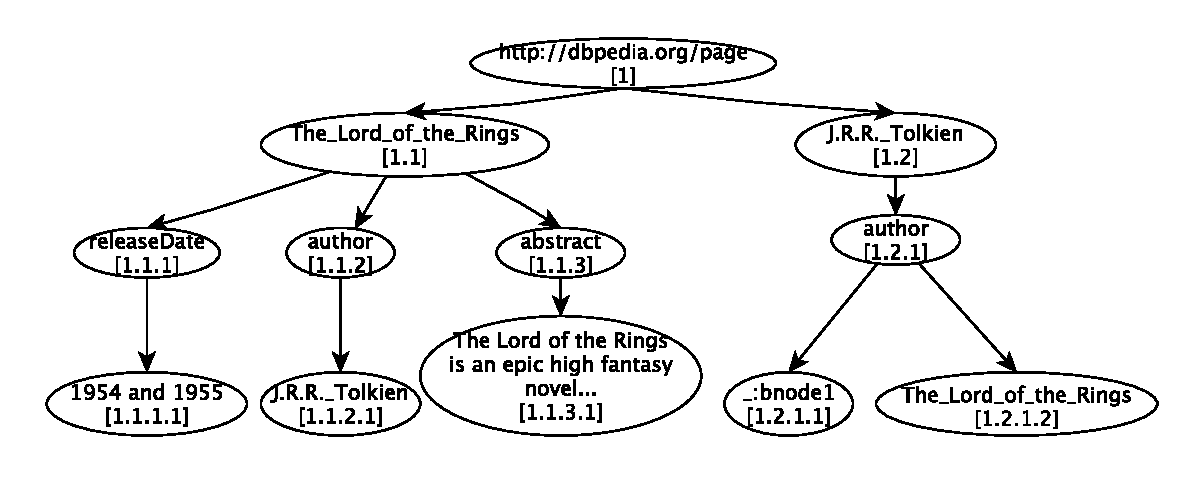
\includegraphics[scale=1]{pics/dewey-encoding}
\label{fig:dewey-encoding}
}}
\caption{The node-labelled tree model.}
\end{figure}

\subsection{Query Model}
\label{sec:siren-query-model}

Entities present a semi-structured structural view, and not a ``bag of
words'' as in traditional search engines. Therefore the query model search
entities with Boolean combinations of attribute-value pairs.

SIREn supports three different types of queries:
\begin{description}
\item[full-text:] traditional keyword query, useful when the schema of the
dataset is unknown;
\item[structural:] complex queries specified in a star-shaped structure, useful
when the data schema is known;
\item[semi-structural:] a combination of the two where full-text search can be
used on any part of the star-shaped query, useful when the data structure is partially known.
\end{description}
These query types provide different level of complexity, depending on the
knowledge of the data structure by the user. But the SIREn engine is aimed to
be used by other machines, and the possibility of complex queries are then
needed. The Figure~\ref{fig:star-query} depicts a star-shaped query that
matches the ``The Lord of the Rings'' entity from the
Figure~\ref{fig:entities}. This semi-structural query makes use of full-text
search through the use of keywords (e.g. ``tolkien'' or ``lord''). We can also
embedded Boolean search inside nodes, then the matching of entities having the
keywords ``lord'' and ``rings'' are marked as a positive match for the value
of an abstract (or label) attribute. The wildcard can also be used to describe
unknown relations between nodes. This search model is developed to find
entities that best match an entity description pattern (e.g. star-shaped
pattern).

In opposite to the full-text logical view where words are seen are seen as a
single bag of words, in the semi-structured view, the words are assigned to
multiple distinct bag of words, one for each value and attribute. Consequently,
it is possible to distinguish when words occur in a same value or different
values and avoid false-positive answers.

\begin{figure}
\centering
\resizebox{0.5\linewidth}{!}{%
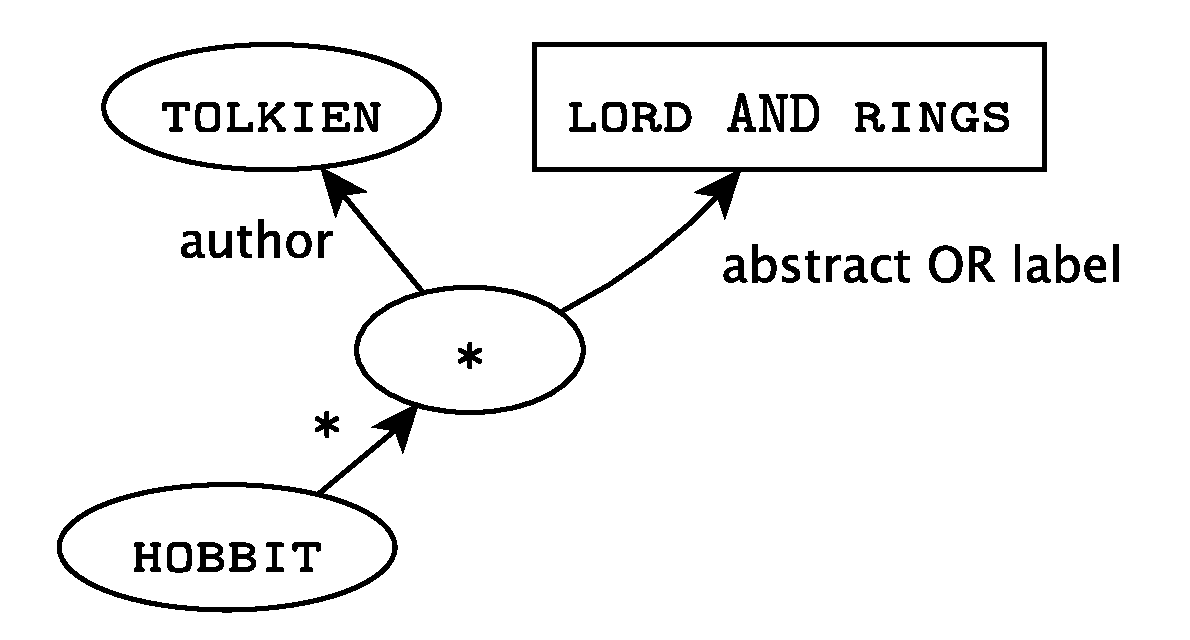
\includegraphics[scale=1]{pics/query}
}%
\caption{A star-shaped query matching the entity ``The Lord of the Rings''
from the Figure~\ref{fig:entities}. The character * stands for the wildcard
variable.}
\label{fig:star-query}
\end{figure}

\section{Model Implementation}

This section aims to present the implementation of the Entity Attribute-Value
model and of the query model over an inverted index. An overview of the
inverted index construction is presented with the entity-centric indexing
before describing more thoroughly the indexing structure.

\subsection{Entity-Centric Indexing}
\label{sec:ent-cent-indexing}

The search unit of the SIREn engine is an entity. As such,
SIREn aims to index entities (i.e., star graphs), and not documents
as the Section~\ref{sec:IR-indexing} presents it.
With a \emph{document-centric} indexing, every terms belong to a same document.
For instance the RDF graph in Figure~\ref{fig:rdf-graph} can be
taken as a whole document, since all data has been taken from the same web page
\url{http://dbpedia.org/page/The_Lord_of_the_Rings}. However when searching for
the entity \emph{The Lord of the Rings}, we just want information about this
entity and not also about any related work. This is a reason why SIREn uses an
\emph{entity-centric} indexing.

With a document-centric indexing, all the terms from the N-Triples of the
Figure~\ref{fig:rdf-graph} are seen as one document.
Then any queries on one of those terms will return that document. With an
entity-centric approach, we index the three different entities separately as
reported in the Table~\ref{tab:TLR-ent-cent}.

\begin{table}
\centering
\resizebox{\linewidth}{!}{%
\begin{tabular}{lc@{\hs}llll}
\toprule
Entity &\phantom{a}& \multicolumn{4}{c}{N-Triples}\\
\cmidrule{3-6}
% \multicolumn{6}{c}{\phantom{a}}\\
{\bfseries TLR} & \multicolumn{5}{c}{\phantom{a}} \\
\multirow{3}{*}{\phantom{a}}&\multirow{3}{*}{\phantom{a}}&
$<$TLR$>$&$<$dbpprop:author$>$&$<$dbpedia:J.\_R.\_R.\_Tolkien$>$&$.$\\
&&$<$TLR$>$&$<$dbpprop:releaseDate$>$&``1954 and 1955''&$.$\\
&&$<$TLR$>$&$<$dbpedia-owl:abstract$>$&``The Lord of the Rings is an
epic\ldots''&$.$\\

{\bfseries \_:bnode1} & \multicolumn{5}{c}{\phantom{a}} \\
\multirow{3}{*}{\phantom{a}}&\multirow{3}{*}{\phantom{a}}&
$<$TLR$>$&$<$dbpprop:precededBy$>$&\_:bnode1&$.$\\
&&\_:bnode1&$<$dbpedia-owl:author$>$&$<$dbpedia:J.\_R.\_R.\_Tolkien$>$&.\\
&&\_:bnode1 &$<$dbpedia-owl:abstract$>$&''The Hobbit, or There and Back
Again is a fantasy novel\ldots''&$.$\\

{\bfseries dbpedia:J.\_R.\_R.\_Tolkien} & \multicolumn{5}{c}{\phantom{a}} \\
\multirow{2}{*}{\phantom{a}}&\multirow{2}{*}{\phantom{a}}&
\_:bnode1&$<$dbpedia-owl:author$>$&$<$dbpedia:J.\_R.\_R.\_Tolkien$>$&.\\
&&$<$TLR$>$&$<$dbpprop:author$>$&$<$dbpedia:J.\_R.\_R.\_Tolkien$>$&.\\

\bottomrule
\end{tabular}
}%
\caption{Entity-centric indexing on ``The Lord of the Rings'' RDF graph of
Figure~\ref{fig:rdf-graph}. Each entity is reported with its star graph in the
N-Triples format.}
\label{tab:TLR-ent-cent}
\end{table}

SIREn stores triples documents into a table where each
documents are stored as rows, a column having a meaning for the
document (e.g. title, abstract, \ldots). The Table~\ref{tab:doc-centric}
reports a document-centric strategy for semantic data like RDF triples, where
the first column stores the triple's subject, the second one the predicate and
the third one the object. As an attribute can be multi-valued, a lot of space is
wasted as three rows are used to store three triples where only the object
changes. In order to save space, thus improving indexing and querying
performances since less data to be written and read, SIREn uses a
representation format called \emph{N-Tuples}. It consists to collapse all
triples with a same predicate into one row and to remove the subject cell, as
depicted in the Table~\ref{tab:ent-centric}.

\begin{table}
\centering
\resizebox{0.8\linewidth}{!}{%
\subfloat[Document-centric indexing.]{%
\begin{tabular}{ccc}
\toprule
$<$ s $>$ & $<$ p1 $>$ & $<$ o1 $>\;.$ \\
$<$ s $>$ & $<$ p1 $>$ & $<$ o2 $>\;.$ \\
$<$ s $>$ & $<$ p1 $>$ & $<$ o3 $>\;.$ \\
$<$ s $>$ & $<$ p2 $>$ & $<$ o4 $>\;.$ \\
\bottomrule
\end{tabular}
\label{tab:doc-centric}
}\quad%
\subfloat[Entity-centric indexing.]{%
\begin{tabular}{cccc}
\toprule
$<$ p1 $>$ & $<$ o1 $>$ & $<$ o2 $>$ &$<$ o3 $>\;.$ \\
$<$ p2 $>$ & $<$ o4 $>$ & $\;.$ & \\
\bottomrule
\end{tabular}
\label{tab:ent-centric}
}}
\caption{Two different indexing strategies for semantic data, e.g. RDF triples.
The characters ``s'', ``p'' and ``o'' refer respectively to the subject,
predicate and object in a triple.}
\end{table}

\subsection{Inverted Index Structure}
\label{sec:siren-inv-lists}

Traditionally in Information Retrieval-based search engines, there are three
streams of integers that form an inverted list. A stream of documents
identifiers, a stream of term frequencies and a stream of positions.
In SIREn there are five stream of integers, being streams of entity
identifiers, of term frequencies, of attributes identifiers, of values
identifiers and of positions, identifiers taken from the Dewey encoding
depicted in the Figure~\ref{fig:dewey-encoding}. The term frequency corresponds
to the number of the term's occurrences in an entity description (e.g. a star
graph). The term position corresponds to the relative position of the term
within its node.

Because of the Dewey encoding, the identifiers numerical values have a
clustering effect: the entity identifier is local to a dataset, and the
attribute identifier is local to that entity, and so on. The
Figure~\ref{fig:siren-inv-lists} depicts the five stream of identifiers that
together form the inverted list in SIREn.
As an example for the locality of identifiers values, the position 5 and 7 in
the entity 10 (i.e., blue squares) describe a same term in a same value node
(i.e., value node with identifier 3). However the green square is local to the
same attribute 5, but not to the same value node.

The repetitive structure of semantic data (e.g. a same URI in the predicate
cell) implies that combining the entity-centric indexing with a delta encoding
of the inverted lists result in a compact inverted index structure. Indeed
because of the locality of the values, the gap between integers will be small.

\begin{figure}
\centering
\resizebox{0.32\linewidth}{!}{%
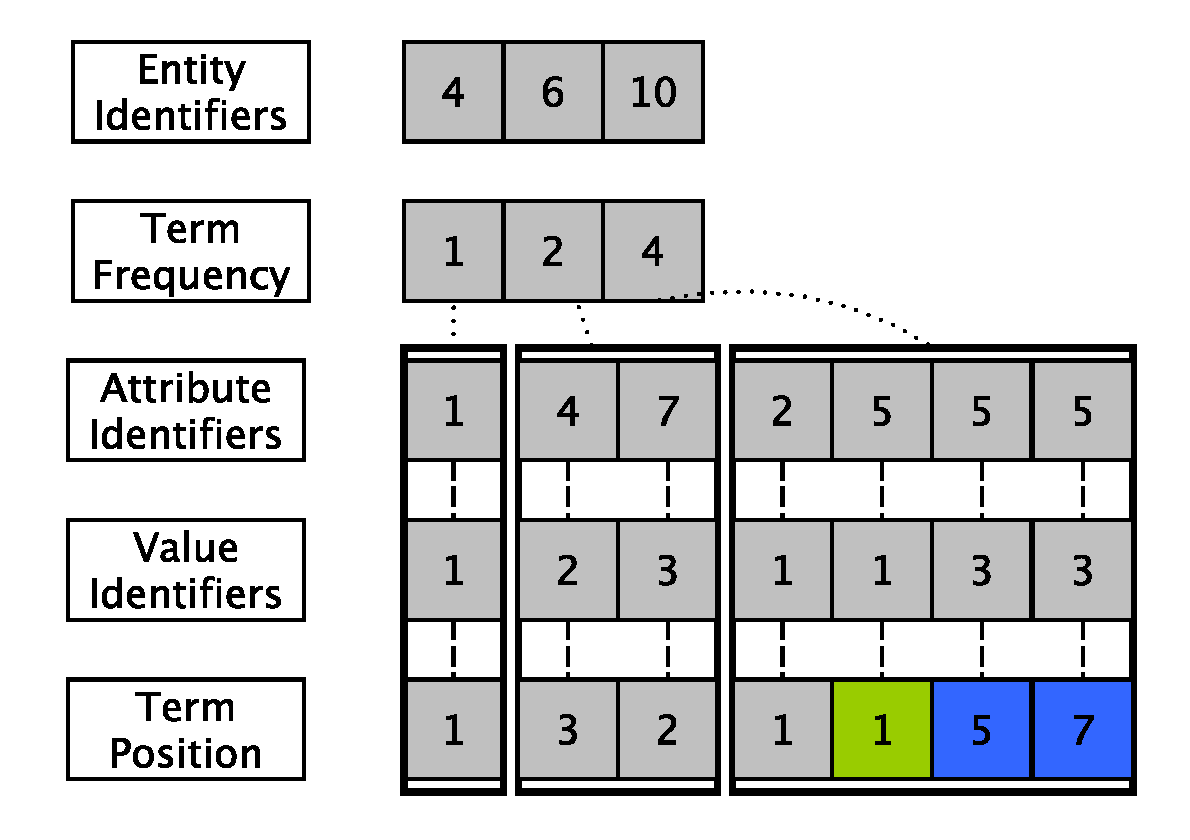
\includegraphics[scale=1]{pics/inverted-list-ex}
}%
\caption{Inverted Lists with the SIREn model.}
\label{fig:siren-inv-lists}
\end{figure}
